\chapter{\color{oxfordblue} The LHC \& ATLAS Experiment}\label{chapter-ATLAS}
\ChapFrame

\textit{
Modern particle physics is at the edge of the technological reach of science. To discover the Higgs boson, an extremely complex infrastuctre is required to probe physics at the required scale. The \gls{lhc} at \gls{cern} is consequently the largest and most powerful particle accelerator and has held this title since its construction in 2008 \cite{LyndonEvans_2008}. It is easily ranks as one of the mox complex machine ever created. Protons are accelerated to up to 99.9999991\% of the speed of light, in a giant 27 km long ring-shaped accelerator, burried 100 m below the surface of the French-Swiss border near Geneva. Superconducting magnets cooled down with liquid helium to 1.9 $K$ steer this energetic beam thanks to powerful magnetic fields of 8.33 Tesla. The beams are made of bunches of particles, collided precisely at four specific interactions points where large detectors are built and operated by dedicated experiments: ATLAS \cite{TheATLASCollaboration_2008}, CMS \cite{TheCMSCollaboration_2008}, ALICE \cite{TheALICECollaboration_2008}, and LHC$b$ \cite{TheLHCbCollaboration_2008}. The first two are multipurpose experiments with overlapping physics programs, while ALICE and LHC$b$ are respectively dedicated to heavy ion and heavy flavour physics. This chapter described the experimental setup of the \gls{lhc} and the ATLAS experiment, focusing on proton-proton collisions and introducing relevant elements to the work presented in this thesis.} 

\section{The Large Hadron Collider}\label{sec-LHC} % TODO check values

\begin{figure}[!h]
  \centering
  \makebox[\textwidth][c]{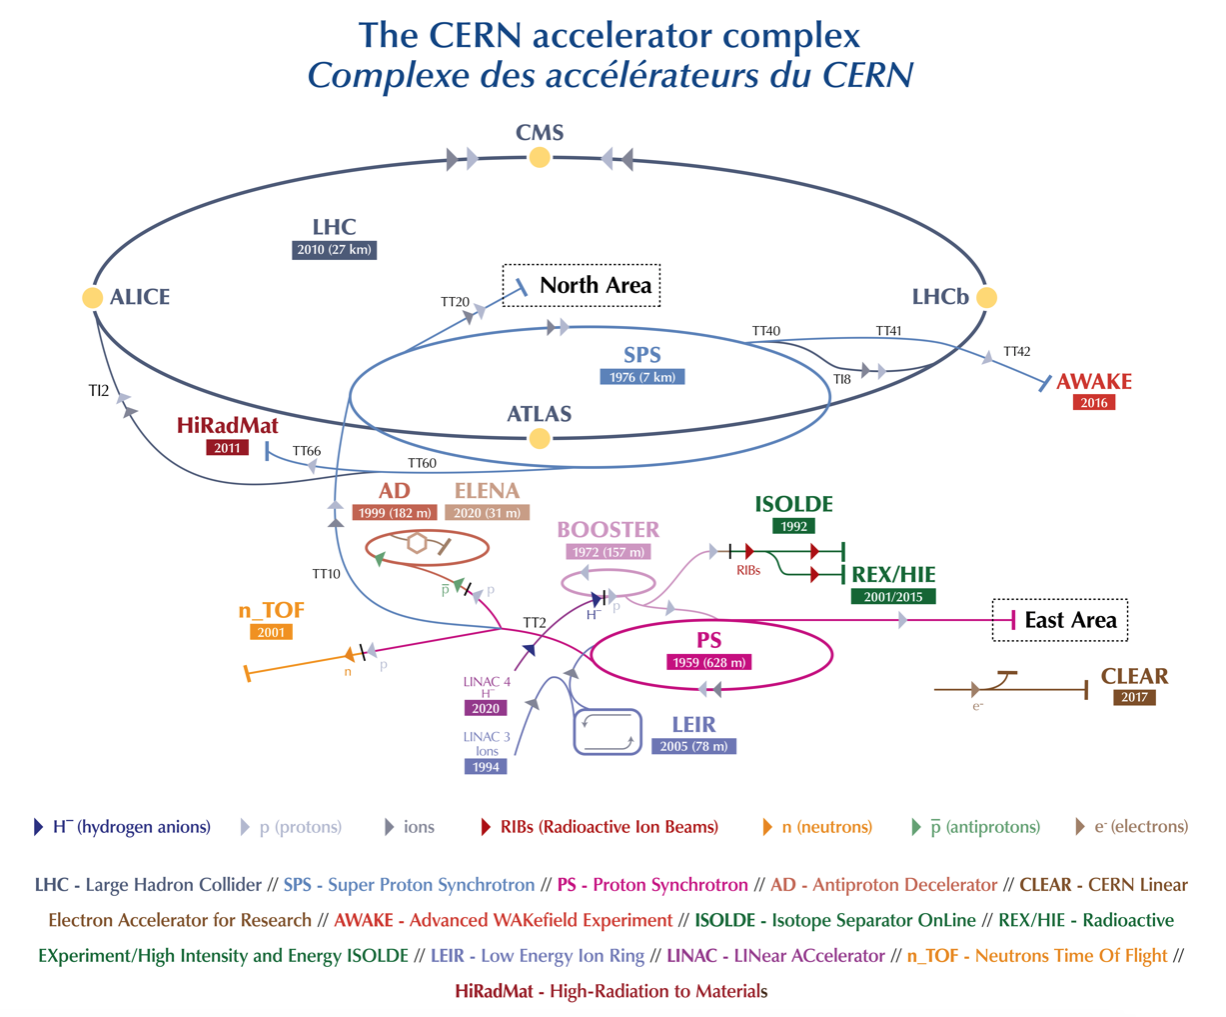
\includegraphics[width=1.05\textwidth]{Images/ATLAS/cernAcc}}
  \caption{The accelerator complex of CERN during Run 3 \cite{CERNAcc}. The LHC is the top dark blue ring.}
  \label{fig-CernAccSys}
\end{figure}

The last machine in a complex multi-stage accelerator complex of CERN displayed in Figure \ref{fig-CernAccSys}, the \gls{lhc} is capable of frontally colliding proton or heavy ion beams. These beams are made of bunches of particles, collided precisely at four interactions points where large detectors are built and operated by dedicated experiments. The life of a proton beam starts innocuously ionised hydrogen $H^-$ gas, passed to a linear accelerator called LINAC4\footnote{Before 2020, it was LINAC2.} to reach energies of 160 MeV. After stripping the ionised hydrogen of its two electrons thus leaving a bare proton, the next acceleration stage is in the Proton Synchroton Booster (BOOSTER) bringing the beam energy to 2 GeV. The protons are then passed to increasingly larger synchrotons: the Proton Synchrotron (PS) to reach energies of 26 GeV, followed by the Super Proton Synchrotron (SPS) to reach energies of 450 GeV. The beam is finally injected into the \gls{lhc} in two different beamlines circulating the proton in opposite directions. Superconducting dipole magnets reaching 8.33 T steer the highly-energetic beams, while complex geometries of magnets (quadrupoles, sextupoles, ...) are deployed to refine the bunch shape through focusing effects. Powerful radiofrequency cavities accelerate them to their final energy of to 6.5 TeV, giving a total $pp$ centre of mass energy of $\sqrt{s} = 13$ TeV in Run 2.  \\

The operation of the \gls{lhc} is split into dedicated \textit{runs} of data taking, separated by \textit{shutdowns} to maintain or upgrade the infrastucture. Some key metrics from these runs from the point of view of the ATLAS experiment are displayed in Table~\ref{tbl:LHCATLASperf}
\begin{table}[!htbp]
    \begin{center}
        \renewcommand{\arraystretch}{1.2}
      %\resizebox{0.99\textwidth}{!}{
        \begin{tabular}{cc|cccc} \hline \hline 
          & Year & $\sqrt{s}$ [TeV] & $\langle \mu \rangle$ &  Luminosity $\mathcal{L}$ [cm$^{-2}$s$^{-1}$] & $\int\mathcal{L}$ [fb$^{-1}$] \\ \hline
          Run 1 & 2010 - 2012 & 7-8    & 18 & 0.8 $\times$ $10^{34}$    & $26.4$ \\
          Run 2 & 2015 - 2018 & 13     & 34 & 1-2 $\times$ $10^{34}$  & $140.1$ \\
          Run 3 & 2022 - 2025 & 13.6     & 50 & 2 $\times$ $10^{33}$    & $65$ \\

          \hline\hline
        \end{tabular}
      %}
      \caption{Metrics on the accerelarator performance of the LHC in the different runs of data taking. The reported values correspond to those recorded by the ATLAS experiment \cite{ATLAS:run1Lumi, ATLAS:2022hro, ATL-DAPR-PUB-2023-001}. Numbers for the ongoing Run 3 are preliminary, with the integrated luminosity listed considering events recorded until July 2023. The number of interactions per bunch crossing averaged over each run is displayed as $\langle \mu \rangle$.} % TODO Define BL and d0
      \label{tbl:LHCATLASperf}
    \end{center}
\end{table}

Run 2 operated at a larger centre of mass energy ($\sqrt{s}$) and higher average instantaneous luminosity $\mathcal{L}$ than Run 1, with Run 3 again pushing up the limits. The average instantaneous luminosity measures the quantity of data collected from the relation
\begin{equation}
  \mathcal{L} = \frac{1}{\sigma}\frac{dN}{dt}
\end{equation}
relating the event rate of a particular process to its cross-section $\sigma$. The instantaneous luminosity is a machine parameter: it depends on the design and the operation of the accelerator. It is calculated from
\begin{equation}
  \mathcal{L} = \frac{N_1N_2N_bf}{4\pi\sigma_x\sigma_y}
\end{equation}
where $N_1$ and $N_2$ are the number of protons in each bunch, $N_b$ the number of bunches, $f$ is the collider revolution frequency, and $\sigma_x$ and $\sigma_y$ are the $x$ and $y$ geometrical extension of the beam density distributions. The integrated luminosity $\int \mathcal{L} dt$ is a direct measure of the quantity of data collected over a certain period, often expressed in units of inverse \textit{barn} b$^{-1}$, where b $= 10^{-28}$ m$^{2}$. For Run 2, the total luminosity recorded corresponds to 140.1 $\pm$ 1.2 fb$^{-1}$, with a small uncertainty of 0.83 \% \cite{ATLAS:2022hro} thanks to a complex measurement involving luminosity-dedicated detectors such as LUCID-2 \cite{Avoni_2018}. Figure \ref{fig-atlasLumiPileup} shows the cumulative total integrated luminosity during Run 2, jointly with another important machine parameter: the average number of interactions per bunch crossing $\langle \mu\rangle$. 

\begin{figure}[!h]
  \centering
  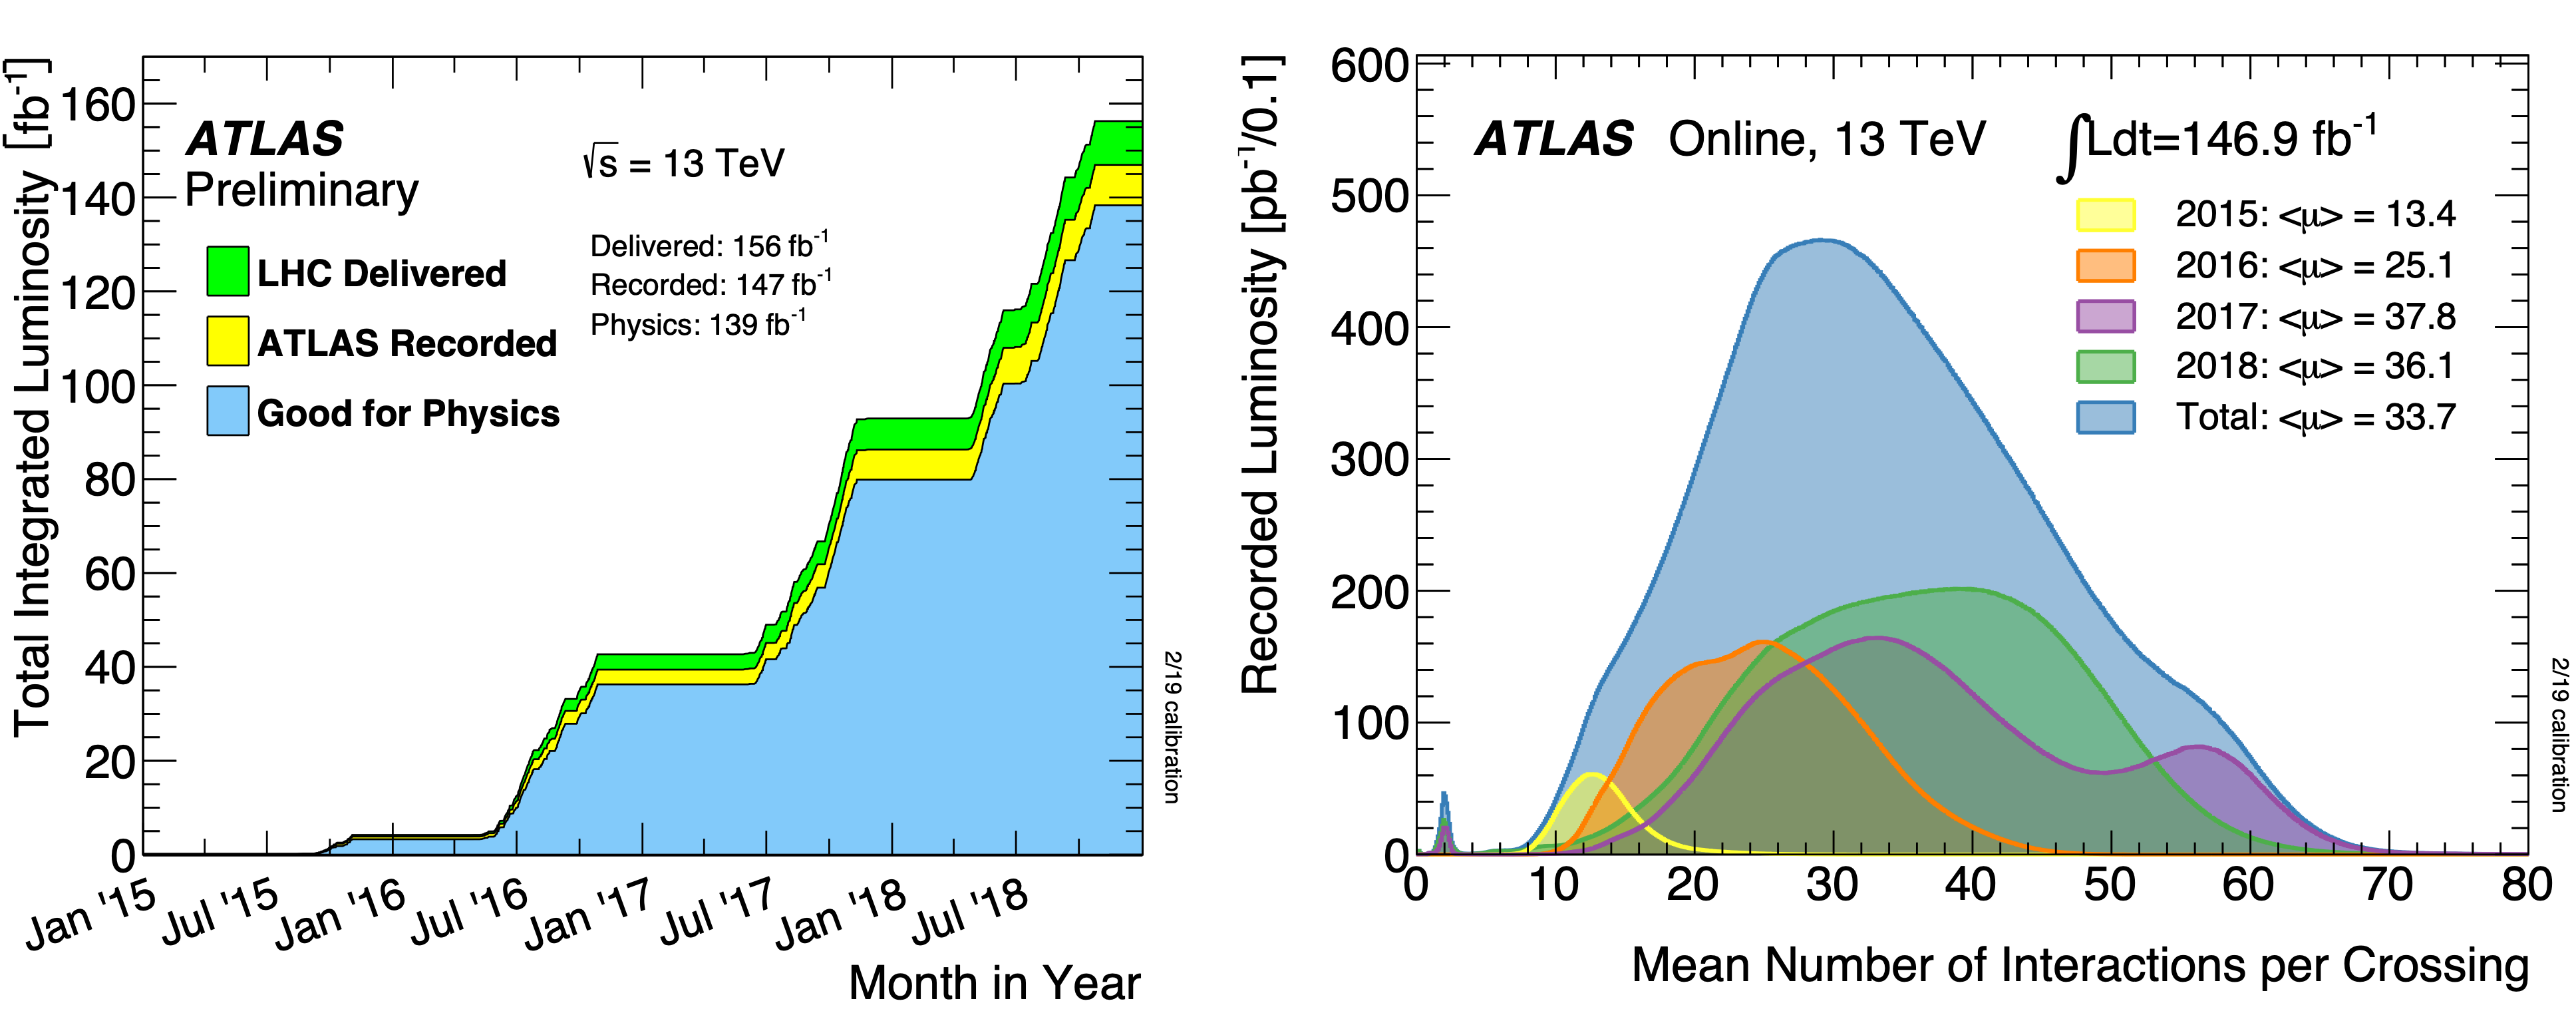
\includegraphics[width=\textwidth]{Images/ATLAS/recoATLAS.png}
  \caption{The ATLAS cumulative integrated luminosity delivered, recorded, and approved for physics (left) and the average pile-up distribution weighted by luminosity (right) during Run 2  \cite{PubAtlasLumi}. The luminosities indicated correspond to an early calculation that was corrected in Ref. \cite{ATLAS:2022hro}.}
  \label{fig-atlasLumiPileup}
\end{figure}

The main event during the collision of the proton bunches is the hard scatter where most of the energy transfer occurs. Other protons in the bunches do have softer interactions leading to background activity called \textit{\gls{pu}}. Two types of pile-up are distinguished: \textit{in-time \gls{pu}} when the soft interaction is from protons in the same bunch as the hard scatter recorded, and \textit{out-of-time \gls{pu}} when the protons are from another bunch crossing. Bunches in the \gls{lhc} are separated by a 25 ns delay, corresponding to a machine frequency of 40 MHz. To control the luminosity, the angle of attack of the beams can be tweaked so that their overlap on the impact point is modified. Having more frontal collisions leads to a larger overlap and  a higher luminosity at the price of more \gls{pu}. 

\section{The ATLAS Detector}\label{sec-ATLASDet}
The ATLAS Collaboration built and operates the eponymous cylindrically shaped multi-layered detector lying 100 m underground with a length of 45 long and a 26 m diameter \cite{TheATLASCollaboration_2008}, as presented in Figure~\ref{fig-AtlasDec}. The experiment is constructed to probe a braod range of physical phenomena, as required from the general purpose of the Collaboration. Aiming to be as hermetic as possible, the detector wraps around the interaction point with the barrel forming the central part of the cylinder and the end-caps closing the geometry at its extremity. Essential characteristics of the design had to be met to manage the extremely high event rate, requiring fast response, radiation-hard sensors, and state-of-the-art readout electronics in combination with good spatial and temporal resolution to disentangle the effect of pile-up. 

\begin{figure}[!h]
\centering
\hspace{-1.25cm}
\makebox[\textwidth][c]{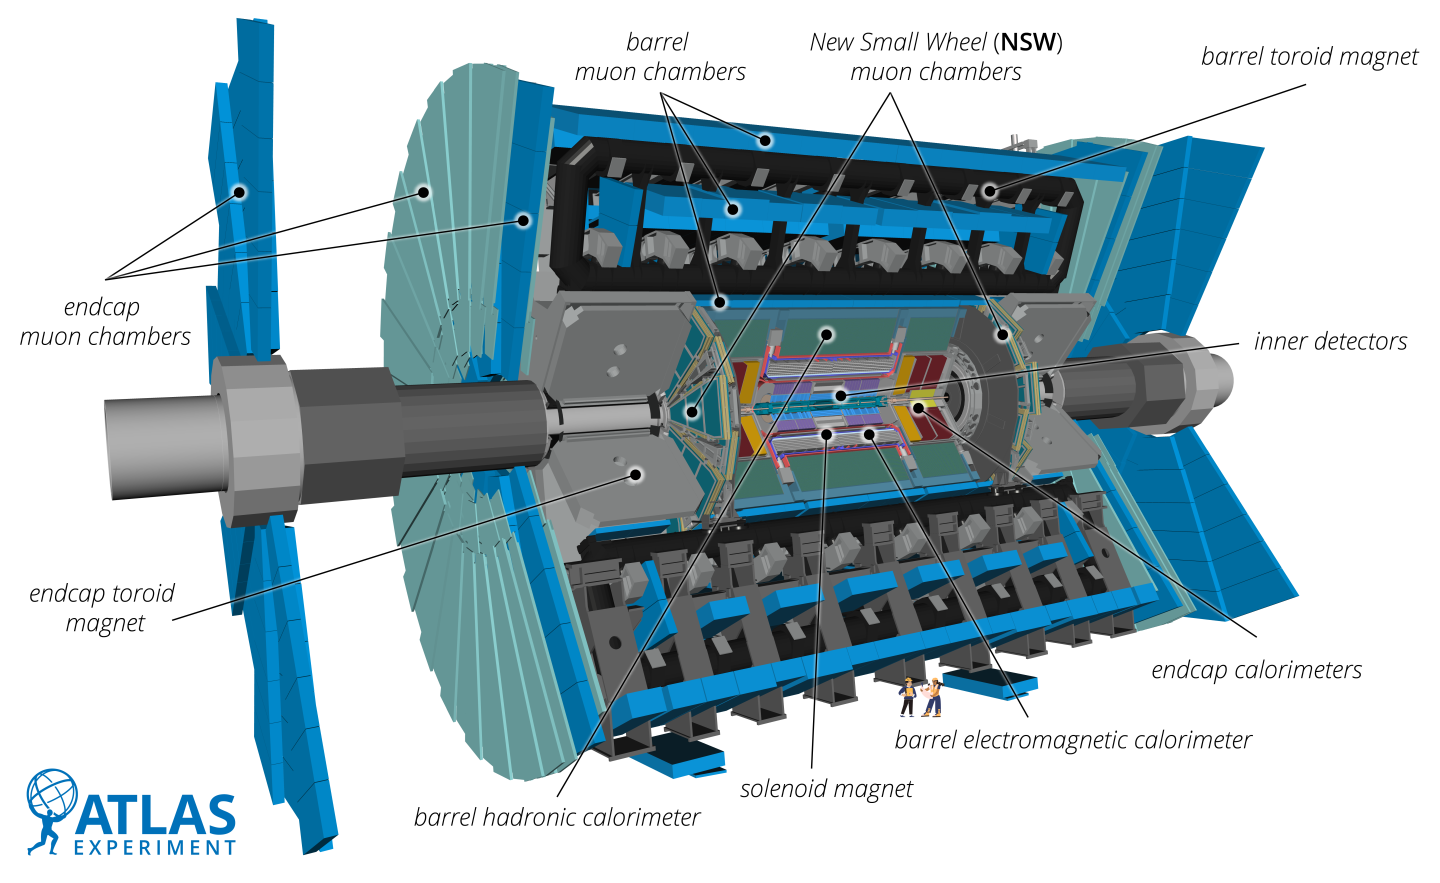
\includegraphics[width=1.08\textwidth]{Images/ATLAS/atlasDet.png}}
\caption{Cut-away view of the ATLAS detector \cite{ATLASschematics}.}
\label{fig-AtlasDec}
\end{figure}

The coordinate system adopted in ATLAS is described in Figure \ref{fig-AtlasCoord}: the $x$-axis point to the centre of the \gls{lhc} ring, the $y$-axis point upwards, and the $z$-axis in the direction of the beamline (anti-clockwise from the top). The azimuthal angle $\phi$ is defined in the transverse plane $x-y$ and the polar angle $\theta$ is measured upwards from the beam-axis (along $y$). Therefore, the transverse momentum \pt\ of a particle is obtained from its momentum vector $\boldsymbol{p} = (p_x, p_y, p_z)$ as: \pt\ $=\boldsymbol{p} \sin\theta = \sqrt{p_x^2 + p_y^2}$. This is of particular interest as the momentum's longitudinal component $p_z$ is not measurable due to the openings for the beamline and the partonic interaction carrying only a fraction of the original proton momentum. Only the transverse momentum can be correctly assessed, as the initial parton is mostly boosted in the direction of the beamline. The rapidity $y$ of a particle, playing a crucial role in the special relativity, is expressed as 
\begin{equation}
  y = \frac{1}{2} \ln \left(\frac{E + p_z}{E - p_z}\right)
\end{equation}
with $E$ and $p_L$ the particle's energy and longitudinal momentum. In the ultrarelativistic limit, when $p >> m$, the rest mass is negligible and $E \approx p$. In such cases, the rapidity $y$ is well approximated by the experimentally reconstructable pseudo-rapidity $\eta$ that is expressed as
\begin{equation}
  \eta = -\ln \left(\tan \frac{\theta}{2}\right).
\end{equation}
Like the rapidity, $\Delta \eta$ is an invariant under Lorents boosts along the longitudinal $z$-axis. It is often combined with the azimuthal angular apperture $\Delta \phi$ to define the angular separation $\Delta R$ between two objets as 
\begin{equation}
  \Delta R = \sqrt{\Delta \phi^2 + \Delta \eta^2} =  \sqrt{\Delta (\phi_2 - \phi_1)^2 + \Delta (\eta_2 - \eta_1)^2}.
\end{equation}

\begin{figure}[!h]
  \centering
  \hspace{+1.5cm}
  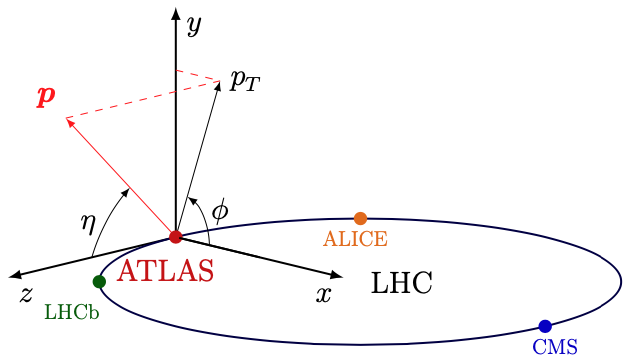
\includegraphics[width=0.6\textwidth]{Images/ATLAS/atlasCoor.png}
  \caption{The ATLAS coordinate system, from \cite{Strong:2020mge}.}
  \label{fig-AtlasCoord}
\end{figure}

As depicted in Figure~\ref{fig-AtlasDec}, ATLAS combines different systems into one precision machine. These subdetectors are able to measure information in the range $|\eta|<  2.5$, with some specialised subdetectors extending further. An essential component in the detector system are its two types of superconducting magnets. Four central solenoid magnets wrap the point of impact and generate a powerful 2 T magnetic field within the inner detectors along the $z$-axis, while toroidal magnets are placed externally on the barrel and the endcaps muon systems to generate a 3.5 T magnetic field deflecting these leptons in the $\eta$-direction. A $q$-charged particles of momentum $p$ is deflected by a magnetic field $B$ due to the Lorentz force, leading to a connexion between the radius of curvature $R$ of the trajectory and the momentum $p$ such as: 
\begin{equation}
  p_{\perp} = 0.3 \, qBR \, [\text{GeV}/c]
\end{equation}
where $p_{\perp}$ is the magnitude of the momentum perpendicular to the magnetic field $\boldsymbol{B}$, and $q$ is expressed in unit of proton charge. Therefore, from the measurement of the curvature, experimentalists are able to infer the component of the momentum transversial to their generated $B$. Higher magnetic fields lead to larger curvature simplifying the measurement of $R$ and improving the resolution of $p_{\perp}$. \\ 

The rest of this chapter reviews the different subdetectors of ATLAS and introduces some common reconstruction methods that are relevant to the work presented in this thesis. 

\subsection{The Inner Detector Tracker}
The detector placed closest to the point of interaction is the \gls{id} \cite{CERN-LHCC-97-016}. This is a tracker covering the range $|\eta| < 2.5$ in a radius of 3 cm to 1 m, designed to record hits in silicon semiconductors or straw-tubes when charged particles fly through so that their trajectory or \textit{track} can be reconstructed from the collected hits. The powerful 2 T magnetic field of the central solenoids enable this detector to measure both charge and momentum. The \gls{id} combines three subsystems, as represented in Figure \ref{fig-AtlasDecID}. 

\begin{figure}[!h]
  \centering
  \hspace{-1.25cm}
  \makebox[\textwidth][c]{\includegraphics[width=1.1\textwidth]{Images/ATLAS/ATLASinDecComb.png}}
  \caption{The Inner Detector of ATLAS \cite{ATLASschematics}.}
  \label{fig-AtlasDecID}
\end{figure}

First, the high-granularity \textit{Pixel Detector} covers the innermost region with three barrel and three endcap layers, for a total of 80 million sensitive semiconductor-based pixels \cite{CERN-LHCC-97-016, Potamianos:2015lar}. During Run 2, an additional \textit{\gls{ibl}} was added at 33 mm from the centre, with 12 million pixels \cite{Capeans:1291633}. This detector gives robust and precise tracking performance and plays a major role in flavour tagging, as described in Chapter~\ref{chap-ftag}. Pixels are 50 $\mu \times$ 400 $\mu$m in the $R\phi \times z$, with a smaller 50 $\mu \times$ 250 $\mu$m for the \gls{ibl}. The current resolution delivered is of 10 $\mu$m (67 $\mu$m) in the transverse $R\phi$ plane ($z$-direction) \cite{Pernegger_2015, ATL-INDET-PUB-2016-001}. \\

The \textit{\gls{sct}} is the next detector, constructed by arranging pairs of silicon microstrips layers into modules assembled into 4 concentric barrel layers and 9 disks in each endcap \cite{AHMAD200798, CERN-LHCC-2017-005}. The resolution is typically of 17 $\mu$m in $R\phi$ and 580 $\mu$m in $z$ \cite{ATLASSCT}. \\

The final system is the \textit{\gls{trt}}, a gas-based straw-tube tracker aiding track reconstruction by delivering numerous hits \cite{TheATLASTRTcollaboration_2008}. Approximately 300 000 drift tubes of a 4 mm diameter filled with a mélange of argon and xenon are arranged along the beamline in the barrel and radially in the endcaps. Each tube has a conducting wire at its centre and its surface is electrically charged, so that a charged particle flying through ionises the gas, leading to a measurable discharge. Polyethylene is place between the tubes to encourage the emission of transition radiation from relativistic particles proportionally to their Lorentz boost $\gamma ~ E / m$. Consequentely, the \gls{trt} is used both for tracking and electron and pion identification, by reconstructing the mass of the charged particles from the amount of $\gamma$-radiation. For tracking, the position resolution provided is of 130 $\mu$m in the $R\phi$ plane for the barrel and the $z-\phi$ plane in the endcaps \cite{Vogel:1537991}. Altogether, the inverse momentum resolution of the ATLAS \gls{id} is
\begin{equation}
  \sigma(1 / p_T) = 0.36 \oplus \frac{13}{p_T \sin\theta} \text{TeV}^{-1}
\end{equation}
where $\oplus$ is the sum in quadrature \cite{TheATLASCollaboration_2008}. This corresponds to a relative error of 0.01\% for a track with \pt\ $\sim$ 500 MeV, and 4\% at a \pt\ $\sim$ 100 GeV.

\subsection{Electronic and Hadronic Calorimeters}
Covering the $|\eta| < 4.9$ region, calorimeters collect the energy of all interacting particles, neutral and charged, except for the muons. They are separated into an electromagnetic calorimeter (ECAL) and a hadronic calorimeter (HCAL) covering jointly the $|\eta| < 3.2$ region and a forward calorimeter for the $3.2 < |\eta| < 4.9$ region, each interlaying specific layers of active and passive materials, as displayed in Figure~\ref{fig-AtlasDecCalo} \cite{\cite{TheATLASCollaboration_2008}}. The passive material typically has a large atomic number to induce cascade of particles called \textit{shower}. The active material, tpyically liquid argon (LAr) collects the energy from these showers through ionisation or scintillation light.\\

The ECAL is designed to collect the energy of electrons and photons, as well as contributing to the measurement of the energy of jets. The active material is LAr and absorbing plates of lead are used as passive material, to encourage bremsstreahlung $e \rightarrow e\gamma$ and pair production from photons $\gamma \rightarrow e^+e^-$. The ECAL have a depth of 22 $X_0$, where the units of \textit{radiation length} $X_0$ track the distance for an electron to have only 1/$e$ its original energy. The energy resolution is parametrised into three terms for the sampling, noise, and a constant contribution, summed in quadrature as \cite{Cavallari_2011}
\begin{equation}
  \frac{\sigma_E^{\text{ECAL}}}{E} = \frac{2.8\%}{\sqrt{E}} \oplus \frac{0.12 [\text{GeV}]}{E} \oplus 0.3\%,
\end{equation}
giving an energy resolution between $\sim$0.5\% for 10 GeV electrons, and $\sim$ 0.6\% for 60 GeV photons.\\

The HCAL is designed to capture the energy of hadronic shower, with LAr as active material for the endcap and forward calorimeters and scintillating plastic tiles for the barrel. As passive material, the endcaps use copper plates, the forward calorimeters use copper and tungsten, and the tile calorimeter in the barrel uses steel. The depth of the hadronic calorimeter is $\sim 10 X$, where $X$ is the nuclear interaction length tracking the average distance before a hadron interacts with a nucleus. The calorimeters collect the majority of the energy, with an HCAL resolution expressed as \cite{Cavallari_2011}
\begin{equation}
  \frac{\sigma_E^{\text{HCAL}}}{E} = \frac{52\%}{\sqrt{E}} \oplus \frac{1.6 [\text{GeV}]}{E} \oplus 3\%.
\end{equation}

\begin{figure}[!h]
  \centering
  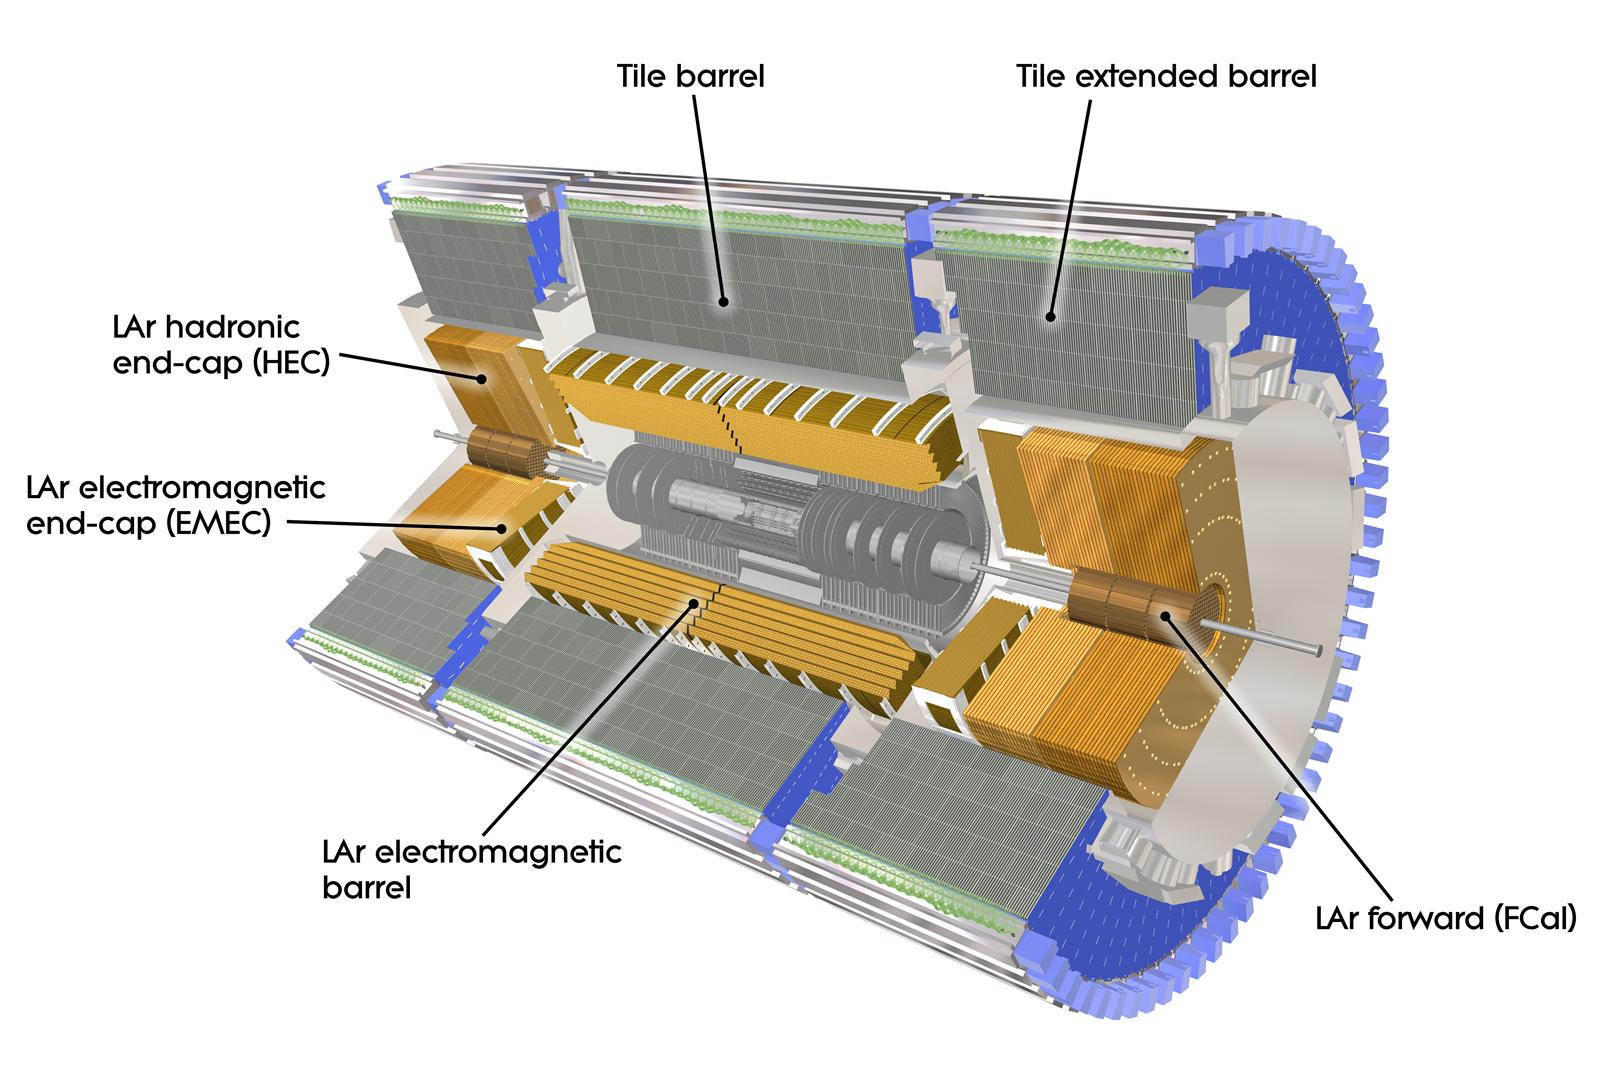
\includegraphics[width=\textwidth]{Images/ATLAS/ATLASCalo.jpg}
  \caption{The calorimeter systems of ATLAS \cite{ATLASschematics}.}
  \label{fig-AtlasDecCalo}
\end{figure}

\subsection{Muon Detection Systems}
Muons require dedicated detection systems to be efficiently and precisely reconstructed in ATLAS. Their high-mass coupled with long lifetime at the energy studied mean they barely interact with the previously described system, only leaving a few hits in the inner detector and flying largely undisturbed through the calorimeters. For this reason, the outmost subdetectors of ATLAS are specially designed to interact with muons. The \gls{ms}, shown in Figure~\ref{fig-AtlasDecMuon}, is a dedicated muon tracking system which also provides an efficient triggering hardware, as described later in this chapter. 

\begin{figure}[!h]
  \centering
  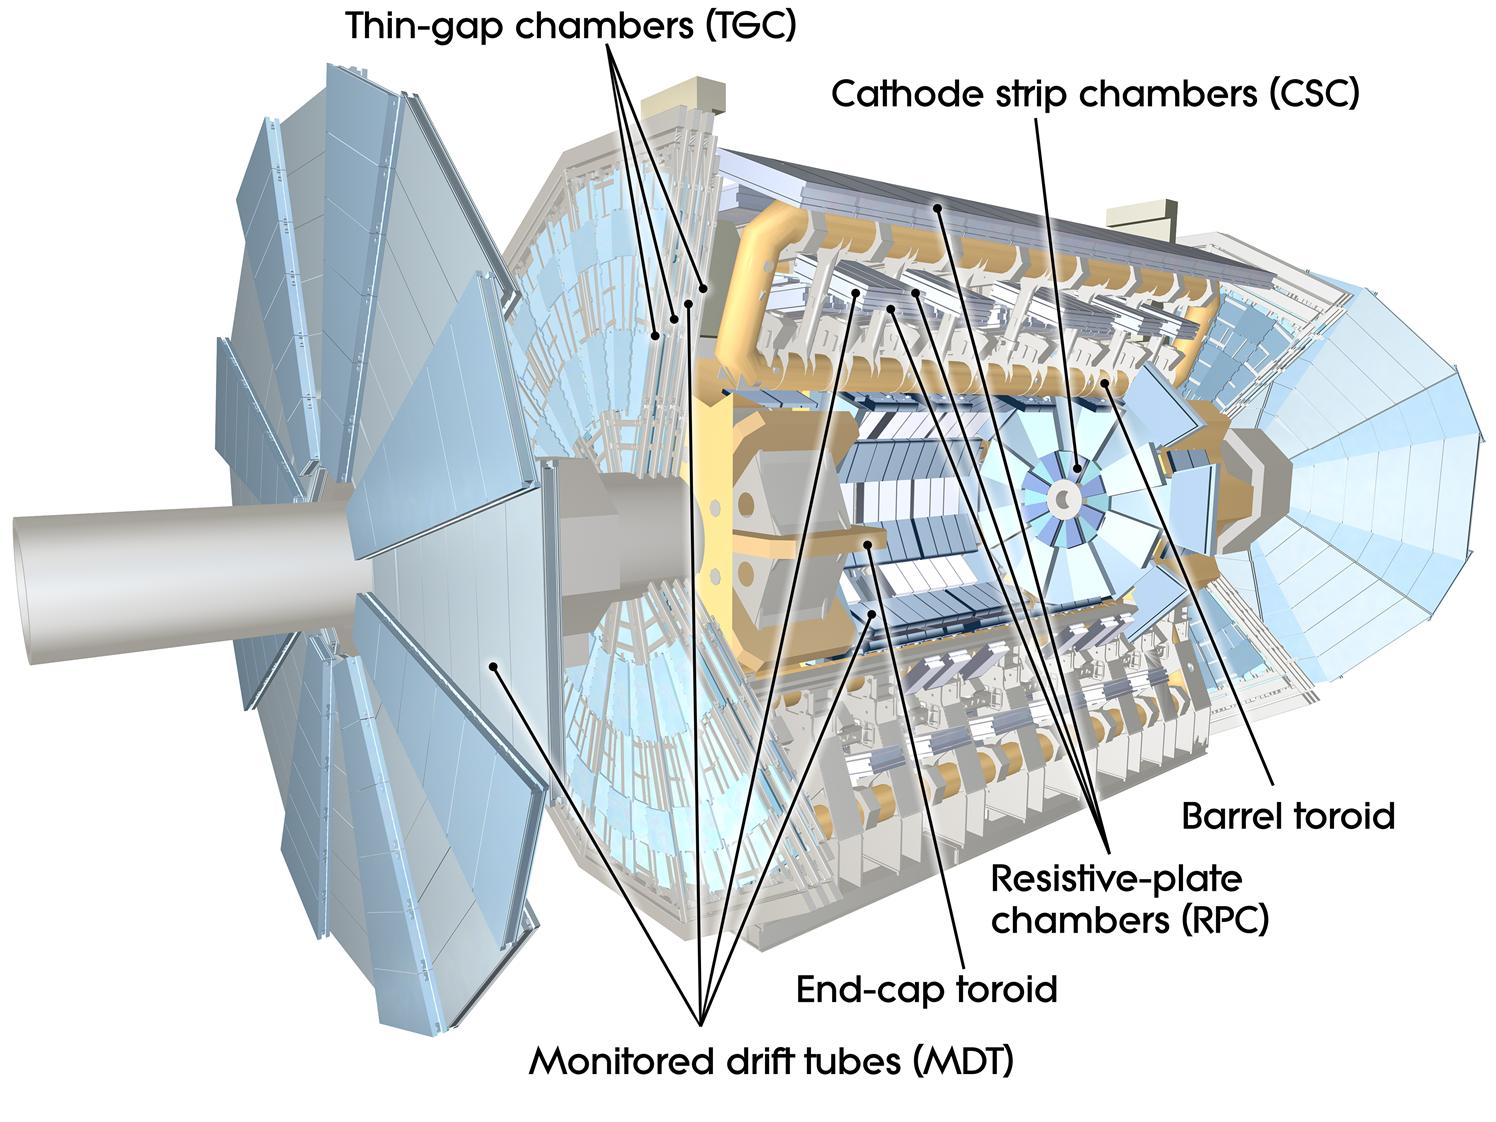
\includegraphics[width=\textwidth]{Images/ATLAS/ATLASMuon.jpg}
  \caption{The muon detectors of ATLAS \cite{ATLASschematics}.}
  \label{fig-AtlasDecMuon}
\end{figure}

The muon tracker is composed of drift tubes split between a barrel region for $|\eta| < 1.2$ and the endcaps $1.2 < |\eta| < 2.7$, with cathore strip chambers in the inner-layers of the endcaps to resist the high activity. The trigger system relies on resitive-plate chambers in the barrel and thin gap chamber in the end-caps. For muon momentum and charge measurements from the tracks, powerful superconducting toroidal magnets are used to deflect muons in the \gls{ms}. The resolution on \pt\ is measured to be of $\sim 1.7$\% (2.3\%) for muons from $J/\psi$ decays in the central (forward) region \cite{atlasMuonPTReco}.

\section{Operation and Reconstruction with the ATLAS Detector}
For physics-quality data taking, the different subdetectors of ATLAS must be performing according to specifications. In operation, the event rate produced by the \gls{lhc} in the heart of the ATLAS detector is of 40 MHz, from the 25 ns bunch-crossing. This unfortunately leads to a data generation rate that is too high for the electronics and computing resource available, requiring the Collaboration to design specific approaches to reduce the rate to a manageable level \cite{Nedden_2017}. This is the task of the trigger system, which is described first in the section. Events that pass the trigger thresholds are stored and must be further processed to reconstruct the physics processes from the low-level measurements performed by the different subdetectors: this is the task of reconstruction, the last subject described in this chapter only for objects types relevant to the presented work. This latter step is performed thanks to the extensive ATLAS software \cite{ATL-SOFT-PUB-2021-001, ATL-SOFT-PUB-2020-001}, exploiting the specific signatures of the different detected particles as schematised in Figure~\ref{fig-ATLASdetect}.

\begin{figure}[!h]
  \centering
  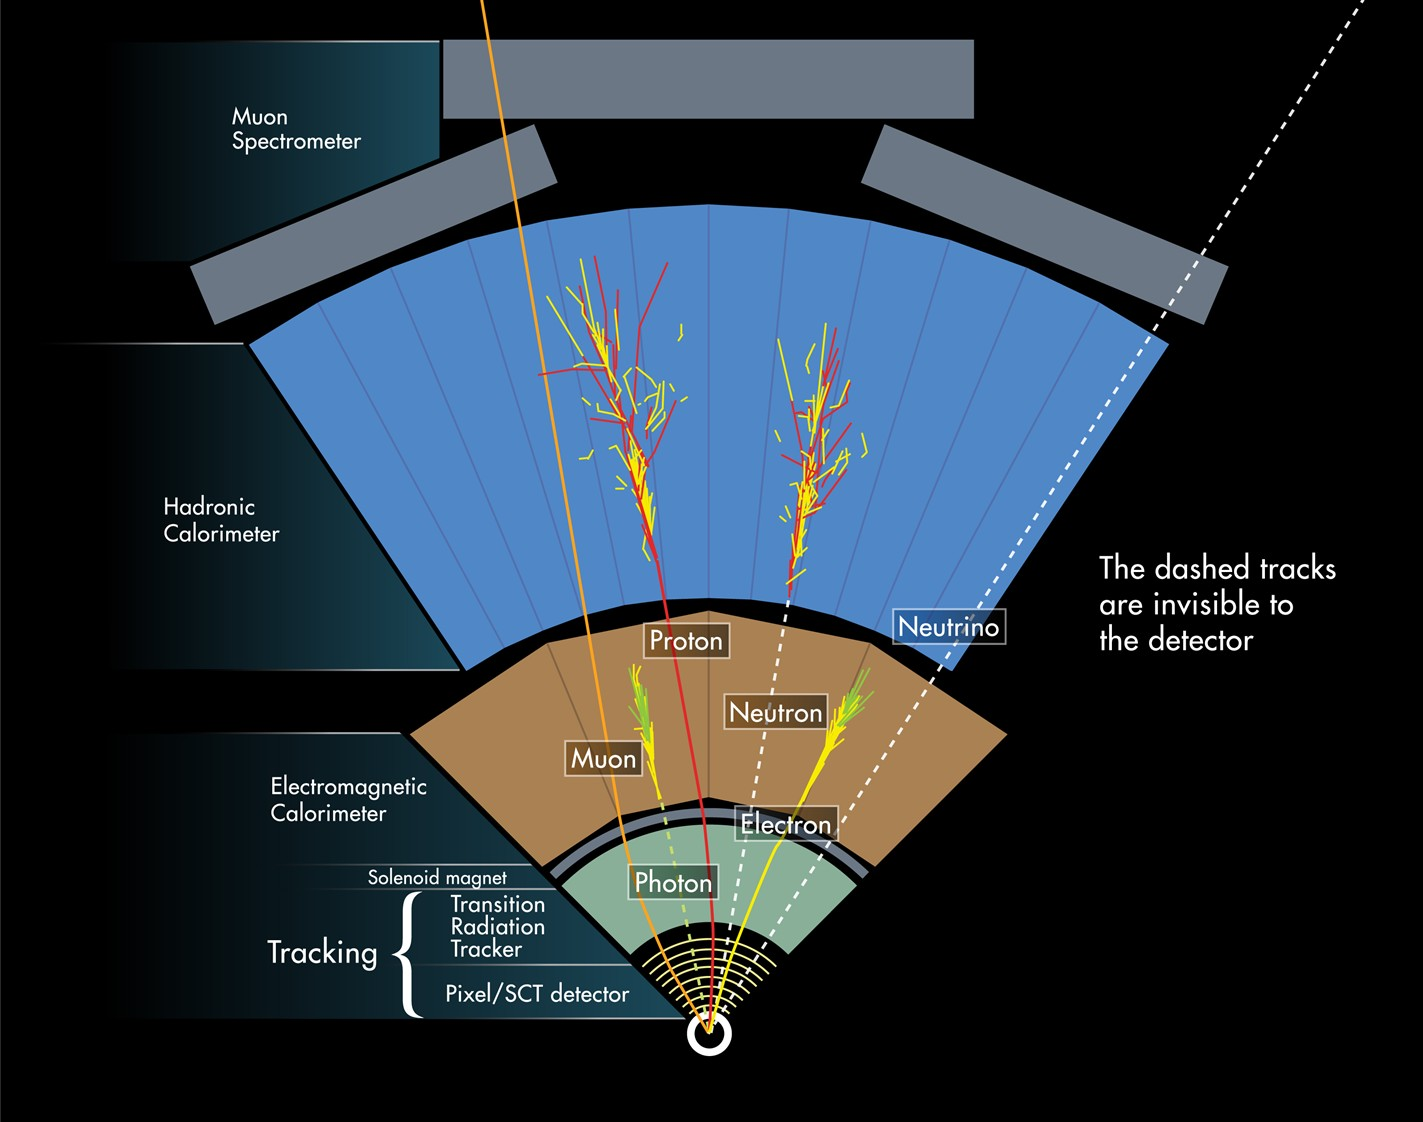
\includegraphics[width=0.8\textwidth]{Images/ATLAS/ATLASdetection.jpg}
  \caption{Schematics of different particles signatures in the ATLAS detector \cite{Pequenao:1505342}.}
  \label{fig-ATLASdetect}
\end{figure}

\subsection{Trigger System}\label{sub-sec-trigger}
The ATLAS trigger system relies on a hierarchical approach to progressively reduce the data rate and select events deemed interesting for physics. Firstly, the \textit{low-level} Level-1 (L1) trigger is built on fast electronic hardware accessing only coarse information to reduce the rate to 100 kHz in $\sim$ 2.5 $\mu$s. This is followed by the High Level Trigger (HLT) that runs on a farm of 40,000 \glspl{cpu} to implement a finer software-based selection, bringing the rate down to a 1.2 kHz or 1.2 GB/s for data storage \cite{TriggerATLAScollaboration_2020}. In this process, gradually more complex information is accessed by dedicated readout and measurement systems. Some commonly used triggers are based on signatures of electrons, muons, missing transverse energy, and $b$-jets. Different trigger menus are designed by the Collaboration, with dedicated data taking period for each setup. Analyses are then able to select data from the whole collected data based on the specific signatures they search. 

\subsection{Low-Level Signatures}
Low-level signatures are used in higher-level reconstruction processes to identify physics objects, such as electrons and jets. Three types are described here: the trajectory of charged particles called \textit{tracks}, the construction of vertices, and the formation of calorimeter clusters. \\

Tracks are the reconstructed trajectory of charged particles through the detector from collected \textit{hits}: localised energy deposits. With denser \gls{pu} activity, the number of hits in a single event becomes significant turning track reconstruction into a challenging computational problem \cite{ATL-PHYS-PUB-2015-006, ATLAS-tracks-algo,}. The trajectories are curved thanks to the previously described superconducting magnets. From a set of hits, tracks are fitted inside-out \cite{ATLAS-tracks-algo}: clusters of three hits in the Pixel or \gls{sct} detectors are first identified as \textit{seeds}, with and additional hits associated by a combinatorial Kalman Filter \cite{10.1115/1.3662552} based on compatibility criteria on the initial track. Hits can initially be shared by several tracks, with the ambiguity resolved later when the reconstructed tracks are ranked by quality and $\chi^2$-fits are performed to quantify the best possible association, favouring high \pt\ tracks. The process is then extended to the \gls{trt} from the oustide-in, and followed by additional quality criteria such as requiring tracks to have a \pt\ > 500 MeV in $|\eta| < 2.5$, a minimum of 7 hits in the Pixex and \gls{sct}, at most one hole, and at most two shared hits. Tracks are parametrised by the longitudinal (along $z$) and transversal (in the $x-y$ plane) \gls{ip}, respectively $z_0$ and $d_0$: these measure the distance from the primary vertex to the perigee of the track\footnote{The point of closest approach of the track with respect to the \gls{pv}.}. \\

Tracks emenate from the decay of particles or radiated through physics processes. If a reconstructed charged particle is produced in the main event, its trajectory leads back to this special location called the \textit{pv} \cite{ATLAS:2016nnj}. If the particle is produced in another decay, the point of emenation can sometimes be distinguished and is labelled \textit{\gls{sv}}. Identifying vertices is crucial for the physics programme of the Collaboration. The primary vertex is identified from a seed vertex first identified from the set of all well reconstructed tracks. The vertex position is then iteratively refined by removing tracks incompatible with the reconstructed vertex and refitting, until some quality criteria are met. Discarded tracks are then used to identify secondary or tertiary vertices. The primary vertex is the one with the largest sum of squared track-\pt. \\

The calorimeters of atlas are composed of many granular layers. So-called clusters are identified by grouping clusters with certain energy deposit measured, either from the \textit{sliding-window} or \textit{topo-clusters} algorithm \cite{Lampl:1099735}. The former one generates fixed-size rectangles by translating the window to maxime the transverse energy $E_T$ measured. The latter clusters neighbouring cells based on a signal to noie criterion. The advantage of the sliding-window is that it is easier to calibrate and is hence used in electron, photon, and hadronic $\tau$'s reconstruction. Topo-clusters are robust against noise and therefore used for jet and missing transverse energy reconstruction.

\subsection{Electrons}
Electrons leave a rich signature in the ATLAS detector, in the \gls{id} and ECAL. For the central region $|\eta| < 2.5$, eletrons are identified and reconstructed with both subdetectors, while the forward region $2.5 < |\eta| < 4.9$ is only covered by the calorimeters with the shape of the shower used to discriminate electrons. Here, only centrally produced \textit{prompt}-electrons are described, where \textit{non-prompt}-electrons are not produced from the main physics process but through later decays or interactions with the detector itself. Photons, pions, and sometimes jets can be mistaken as electrons, with identification and isolation criteria derived to provide high purity and efficiency samples to analyses. Reconstruction relies on calorimeter clusters and track information. When relevant, tracks are matched to the clusters based on the expected energy loss. The track is also extrapolated to insure compatibilty with the cluster barycentre. The process is re-ran with more stringent conditions after refitting the tracks matched to clusters, so that energy loss is taken into account. A prompt-electron is required to have a track matched to the \gls{pv}. The absence of a precision hits or a matched track leads to consider the calorimeter clusters as a photon deposit. \\

To further discriminate prompt-electrons from non-prompt electrons and photons, which act as a background due to photon conversion to $e^+e^-$, a likelihood-based identification algorithm built on a \glsfirst{mva} is deployed \cite{Aaboud:2657964}. Parameters used include the number of hits in each tracker layer, the \glspl{ip}, a calorimeter cluster parameters. Several working points that are progressively more selected are defined on the discriminant, from \textit{Very Loose}, \textit{Loose}, \textit{Medium}, to \textit{Tight}. Prompt-electron candidates are required to be isolated from other tracks and other energy deposits, with specific criteria that are either \gls{id}- or calorimeters-based. In the former case, the sum of tracks \pt\ in a $\Delta R$ cone around the electron is used, while the latter analyses the sum of energy deposit in a calorimeter cone around the electron cluster. As further described in Chapter~\ref{sec-unc}, the efficiency of the electron reconstruction, including identification and isolation, are computed by comparing the measured and simulated measurements of the $Z\rightarrow e^+e^-$ and $J\psi\rightarrow e^+e^-$. Photons are reconstructed similarly to electrons, with no tracks being matched for unconverted photons. Converted photons are allowed hits in the \gls{id}. 

\subsection{Muons}
The \gls{ms} is the main detector to reconstruct muons, with other subdetectors playing a smaller role: muons can indeed leave a track in the \gls{id} and some energy deposits in the calorimeters. These fragmented signatures in the subdetectors are combined to identify muon candidates. In the \gls{ms}, tracks are constructed from a fit of the sucessive hits in the different chambers. \textit{Combined muons} are defined by matching a track in the \gls{ms} to a track in the \gls{id}, with additional information from the calorimeters. Prompt-muons are rejected from background-produced muons (such as in the decay of a $b$-hadron) by specific criteria targeting discrepancies in the \pt between the \gls{ms} and \gls{id}. Increasingly selective working points are defined to identify muons as \textit{Loose}, \textit{Medium}, \textit{Tight}, \textit{High-\pt}. Isolation requirements are applied similarly to the electron case, either track- or calorimeter-based in a $\Delta R$ cone around the candidate muons. The calibration of muons is performed similarly to the electrons, on a $Z\rightarrow \mu^+\mu^-$ and $J\psi\rightarrow \mu^+\mu^-$ samples.

\subsection{Jets}
Quarks and gluons are the most commonly produced particles in a hadron collider setting. As described in Chapter~\ref{chap-theory}, these particles carry colour-charges and undergo hadronisation when produced to neutralise their free colour. This complex process leads to a unique signature in the detector: a spray of particles emitted within the original parton direction called a \textit{jet}. Electrically charged and neutral particles are contained within jets, with most of their energy deposited in the hadron calorimeters. These aggregated objects are therefore constructed by applying a clustering algorithms on tracks and/or calorimeter clusters, depending on the jet defintiion. The most notarious clustering method is the anti-$k_T$ algorithm, thanks to the robustness of the defined jet to collinear splitting or additional soft emissions \cite{Cacciari:2008gp}. The algorithm starts by considering high momentum object, to which softer objects are added thus growing the clusters. Two measures of distances $d$ are used as parameters when considering whether to cluster object $i$ and $j$:
\begin{equation}
  d_{ij} = \min\left(\frac{1}{k_{Ti}^2}, \frac{1}{k_{Tj}^2} \right) \frac{\Delta R_{ij}^2}{R^2},
\end{equation}
and
\begin{equation}
  d_{iB} = \frac{1}{k_{Ti}^2}.
\end{equation}
The first distance, $d_{ij}$, combines the angular apperture $\Delta R_{ij}$ between $i$ and $j$\footnote{$\Delta R_{ij}^2 = (\eta_i - \eta_j)^2 + (\phi_i - \phi_j)^2$.} with the transverse momentum $k_T$ of the two objects and a fixed \textit{radius} parameter $R$. This distance defines a jet radius limiting the size of the associated cone. It is compared to the second distance, $d_{iB}$, assessing the size of the already formed cluster $i$. If $d_{ij} < d_{iB}$, $j$ is clustered with $i$, otherwise $i$ is identified as a jet and removed from consideration. The algorithm proceeds after updating the distances, until all constituents are assigned a cluster. Typical radius values for ATLAS are $R = 0.4$ and $R=1.0$, defining respectively small-$R$ and large-$R$ jets. The former is commonly used for quark and gluon jets, while the latter is employed by analysis to identify boosted heavy objects decay, such as $W$ or Higgs bosons. \\

Jets can be constructed from tracks, calorimeter clusters, or both. In ATLAS, several types of jets are deployed, depending on the desired properties and the objects they are meant to represent. The following types are all reconstructed with the anti-$k_T$ algorithm, clustering different objects:
\begin{itemize}[leftmargin=*]
\item PFlow jets are reconstructed from particle-flow objects \cite{atlasPFLOWjet} with a radius $R$ = 0.4. These objects combine tracking information from the \gls{id} to the calorimeter clusters, leading to a better energy resolution at low \pt\ and lower \gls{pu} contamination after calibration \cite{PhysRevD.96.072002}.
\item EMTopo jets are constructed from denoised topological calorimeters clusters called \textit{topoclusters}, based on the per cell energy sigificance $S_{\text{cell}} = E_{\text{cell}} / \sigma_{\text{cell}}$, where $E_{\text{cell}}$ is the energy and $\sigma_{\text{cell}}$ the expected noise level in the cell \cite{atlasEMTOpo}. The topoclusters are then used with the anti-$k_T$ method with a small 0.4 or large 1.0 radius.
\item Large-$R$ jets are built from topological calorimeter clusters with a radius $R = 1.0$. These jets are applied trimming to remove the contribution from soft contamination, which is mainly due to \gls{pu} and \gls{ue} activity, leading to an improved mass resolution \cite{ATLAS:largeRjet}
\item Track-jets are constructed are based on the anti-$k_T$ clustering algorithm with a variable radius $R$ depending on jet \pt, such that the wide cone used at low \pt\ ($R \approx 0.4$) becomes narrower at high \pt\ ($R \approx 0.02$). They are typically matched as sub-jets of a large-$R$ jet, to deploy the flavour tagging techniques described in Chapter~\ref{chap-ftag}.
\end{itemize}
PFlow and variable-radius jets are used to train the algorithms of Chapter~\ref{chap-ftag}, while EMTopo, large-$R$, and track jets are used in the analysis of Chapter~\ref{chap-VH}. Jets can be assigned a flavour based on the presece of an original parton within a $\Delta R = 0.3$ cone around the jet axis. Experimentally, the flavour is often determined based on the hadrons associated to the jet, as described in detail in Chapter~\ref{chap-ftag}. \\

Jets benefit from extensive calibration to correct the reconstructed properties such as the mass, the energy, and the jet axis direction. In particular, corrections to account for \gls{pu} activity and out-of-cone emissions and deposits are considered. Detector effects are also taken into account, such as differences between the electromagnetic and hadronic calorimters and leakage out of the active regions. The so-called \textit{\gls{jes}} calibrations corrects the jets in successive steps \cite{ATLASjesjerMeas}: 
\begin{itemize}[leftmargin=*]
\item \textit{Origin}: the jet axis, initially constructed from the centre of ATLAS, is corrected to point from the \gls{pv}, and the \pt\ is updated.
\item \textit{Pile-up}: both in-time and out-of-time pile up leave additional energy deposit in the calorimeters. This is substracted from the jet, from first an overall estimation based on the average pile-up and then from the actual number of interactions and vertices in the event. 
\item \textit{Absolute}: absolute energy corrections dependent of the energy $E$ and $\eta$ are derived toto match the data energy scale to the particle-level energy scale of dedicated simulated samples.
\item \textit{Eta inter-calibration}: the detector is not homogenous and the forward regions measurements are typically less accurate. Corrections to these forward jets are applied based on central jets ($|\eta|<1.4$).
\item \textit{Global sequential calibration}: energy leakage in the calorimeters is accounted for with a set of four-momentum Corrections based on five different observables tracking the shape and the energy of the jet.  
\item \textit{In-situ calibration}: corrects any possible differences due to an incorrect description of the detector in the simulations by performing a fit to data a dedicated measurement of a well reconstructed object. Events from the following processes are used in increasing \pt\ scales: $Z+$jet events with the $Z$ leptonically decaying, $\gamma$+jet, and \gls{qcd} multi-jet events at high momentum.
\end{itemize}
The \gls{jes} is parametrised by \pt, and dedicated uncertainties are derived for analyses to use. The \textit{Jet Energy Resolution (JER)} is then defined as $\sigma_{p_T}/p_T$, and also calibrated with dedicated uncertainties derived from a fit to di-jet events \cite{ATLASjesjerMeas}. Despite the \gls{jes} correction procedure, \gls{pu} jets can be still significant and a dedicated \gls{jvt} is used to reject this background \cite{ATLAS-CONF-2014-018}. This implements a 2D likelihood method built from tracking variables from which different selection criteria are derived as working points with specific \gls{pu} jet rejections. 

\subsection{Taus}
Taus make the heaviest generation of the charged lepton, with a mass of 1.8 GeV slightly higher than that of $c$-quarks \cite{Tanabashi:2018oca}. Their lifetime is so short they mostly decay within the beampipe. They leptonically decay to neutrinos and a $e$ or a $\mu$ 35\% of the time, while the rest occurs hadronically. The leptonic decays are hard to disentangle from prompt electrons and muons. Hadronic decays however leave a signature reconstructed as a small-$R$ jet in ATLAS. These hadronic taus are identified by a \glspl{rnn}, to disentangle them from \gls{pu} and \gls{qcd} jets \cite{ATL-PHYS-PUB-2019-033}. This discriminant is used with specific working points derived to define different efficiencies. 

\subsection{Missing Transverse Energy}
Some physics objects do not interact with the ATLAS detector, such as neutrinos and hypothetical \gls{bsm} particles. Consequentely, their presence is not detectable but can be inferred thanks to the negligible initial \pt\ of the two interacting partons in the proton-proton collision. Requiring the transverse energy and momentum to be balance to 0, the so-called \textit{Missing Transverse Energy \etm} or \textit{MET} is calculated as the negative vectorial sum of all physics object transverse momentum
\begin{equation}
  \boldsymbol{E}_T^{\text{miss}} = - \sum_{\text{hard}} \boldsymbol{p}_T - \sum_{\text{soft}} \boldsymbol{p}_T,
\end{equation}
where the sum is decomposed into a \textit{hard} term englobing all physics objects (photons, electrons, muons, taus, and jets) and a soft term including good-quality \gls{id} tracks associated to the \gls{pv} but not to a physics object \cite{ATLASmetReco}. The performance of the reconstruction is measured by comparing simulations to data, with scale and resolution derived with uncertainties to be used by physics analyses. 